\section{Java Enterprise Edition}

Java Enterprise Edition (JEE) is a platform designed for the creation, deployment, and maintenance of three-tier web applications.
\begin{figure}[H]
    \centering
    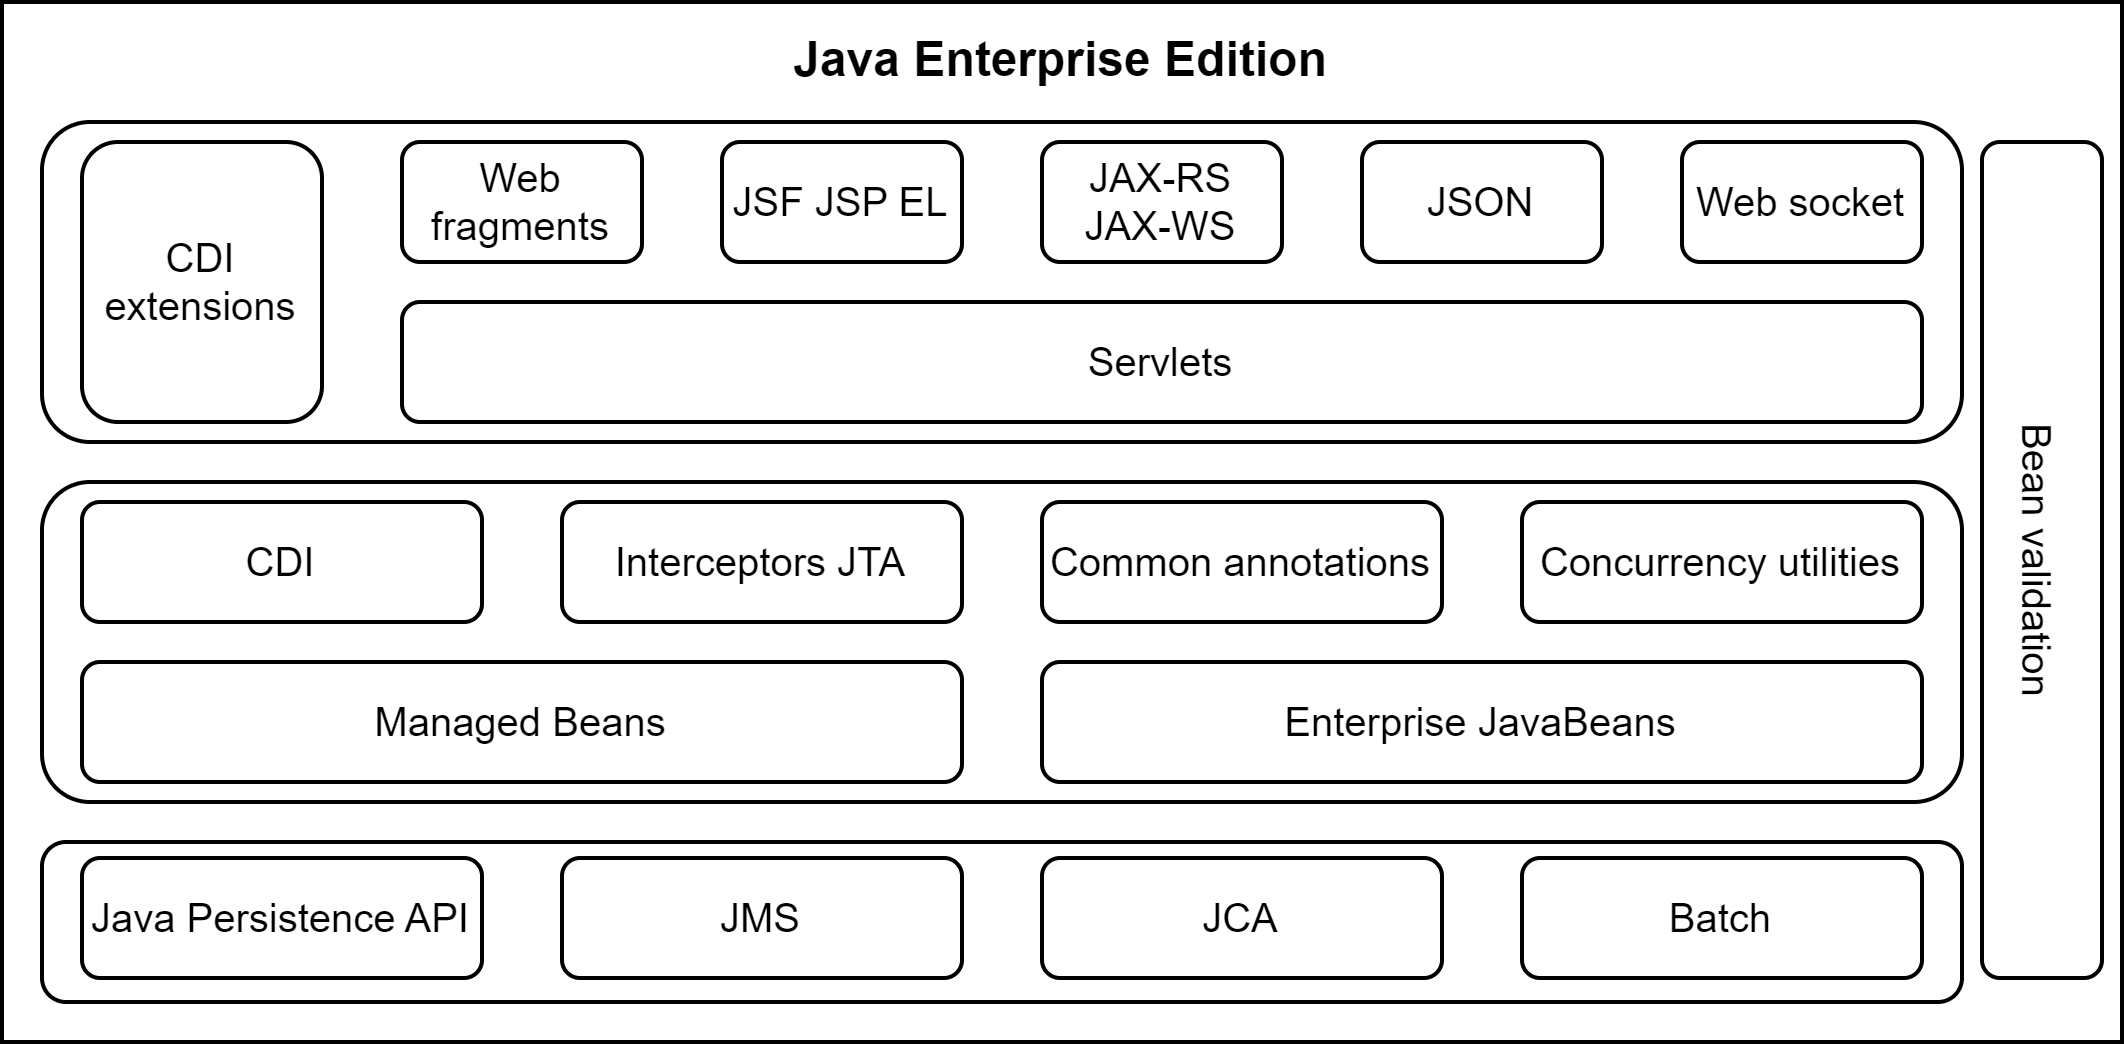
\includegraphics[width=0.75\linewidth]{images/jee.png}
\end{figure}
JEE comprises the following elements:
\begin{enumerate}
    \item \textit{Java Database Connectivity} (JDBC): this is the initial industry standard for establishing database-independent connectivity between Java and databases. 
        JDBC allows establishing connections with databases, sending SQL statements, and processing the results.
    \item \textit{Servlets}: these are Java technologies used in the presentation tier of web applications. 
        Servlets offer a platform-independent, component-based approach for constructing web-based applications. 
        They have access to other Java APIs for interfacing with enterprise databases and operate within a container for concurrency control and lifecycle management.
    \item \textit{Enterprise Java Beans} (EJB): EJB enables the development of distributed, transactional, secure, and portable applications.
        EJB components facilitate interaction between the web front-end and business functions, as well as data access services.
    \item \textit{Java Persistence API} (JPA): JPA defines an interface for mapping relational data to objects in Java.
    \item \textit{Java Transaction API} (JTA): JTA manages transactions in Java, allowing components to initiate, commit, and roll back transactions in a resource-agnostic manner. 
        With JTA, Java components can oversee multiple resources within a single transaction using a unified interaction model.
\end{enumerate}